%%%%%%%%%%%%%%%%%%%%%%%%%%%%%%%%%%%%%%%%%%%%%%%%%%%%%%%%%%%%%%%%%%%%%%%%%%%%%%%%%%
\begin{frame}[fragile]\frametitle{}
\begin{center}
{\Large About Me}
\end{center}
\end{frame}

%%%%%%%%%%%%%%%%%%%%%%%%%%%%%%%%%%%%%%%%%%%%%%%%%%%%%%%%%%%
\begin{frame}[fragile]\frametitle{Yogesh Haribhau Kulkarni}
\begin{columns}
    \begin{column}[T]{0.7\linewidth}
		Bio:
      \begin{itemize}
		\item 20+ years in CAD/Engineering software development
		\item Got Bachelors, Masters and Doctoral degrees in Mechanical Engineering (specialization: Geometric Modeling Algorithms). 
		\item Currently doing Coaching in fields such as Data Science, Artificial Intelligence Machine-Deep Learning (ML/DL) and Natural Language Processing (NLP).
		\item Feel free to follow me at:
      \begin{itemize}
			\item Github (github.com/yogeshhk)
			\item LinkedIn (www.linkedin.com/in/yogeshkulkarni/)
			\item Medium (yogeshharibhaukulkarni.medium.com)
			\item Send email to yogeshkulkarni at yahoo dot com
			\end{itemize}
	  \end{itemize}
    \end{column}
		
    \begin{column}[T]{0.3\linewidth}
      \centering
      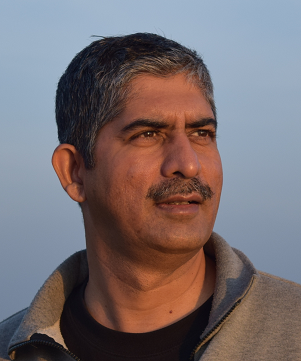
\includegraphics[width=0.8\linewidth,keepaspectratio]{myphoto}
			
			Office Hours: Saturdays, 2 to 5pm (IST); Free-Open to all; email for appointment.
    \end{column}
		
  \end{columns}

\end{frame}


% %%%%%%%%%%%%%%%%%%%%%%%%%%%%%%%%%%%%%%%%%%%%%%%%%%%%%%%%%%%
% \begin{frame}[fragile]\frametitle{Work Done So Far (recently)}
% \begin{columns}

    % \begin{column}[T]{0.4\linewidth}
	% Projects:
      % \begin{itemize}
		% \item Lawyer Assistant: Mining court judgments, topics, doc similarity and summarization.
		% \item Pharmacovigilance: Clinical Medical Healthcare Pharma drug-AE (Adverse Event) detection
		% \item Smart Home Automation: Predictive Analytics, Internet Of Things (IoT)
		% \item ChatBot: FAQ chat bot for GST (Goods and Services Tax) related queries.
	  % \end{itemize}

    % \end{column}
    % \begin{column}[T]{0.6\linewidth}
	% Trainings:
      % \begin{itemize}
		% \item Programming with Python: Basic + Advanced (16 hrs)
		% \item Machine Learning with Scikit-Learn (24 hrs)
		% \item Natural Language Processing with Nltk (16 hrs)
		% \item Deep Learning with Keras/Tensorflow (8 hrs)
		% \item Chatbot Development with Rasa (8 hrs)
	  % \end{itemize}
	  % On-line Courses:
      % \begin{itemize}
		% \item ``Dimension Reduction'' : Experfy
		% \item ``Hands on Capstone Project'' : Experfy 
		% \item ``Introduction to Machine Learning'' : INE
	  % \end{itemize}	  
    % \end{column}
  % \end{columns}
% \end{frame}


% %%%%%%%%%%%%%%%%%%%%%%%%%%%%%%%%%%%%%%%%%%%%%%%%%%%%%%%%%%%%%%%%%%%%%%%%%%%%%%%%%%
% \begin{frame}[fragile]\frametitle{}
% \begin{center}
% {\Large My thoughts on AI, ML/DL, NLP \ldots}
% \end{center}
% \end{frame}

% %%%%%%%%%%%%%%%%%%%%%%%%%%%%%%%%%%%%%%%%%%%%%%%%%%%%%%%%%%%%%%%%%%%%%%%%%%%%%%%%%%
% \begin{frame}[fragile]\frametitle{AI for what?}
% \begin{itemize}
% \item Machines replaced muscles, because just muscles were not scalable for mass production. Thats the automation that happened in Industrial Revolution.
% \item AI is replacing mind/intelligence now, because human intelligence is not scalable for complex decision making, especially if it needs to consider millions for data sources. Thats the automation happening with Machine/Deep Learning using Data.
% \end{itemize}
% \end{frame}

% %%%%%%%%%%%%%%%%%%%%%%%%%%%%%%%%%%%%%%%%%%%%%%%%%%%%%%%%%%%
% \begin{frame}[fragile]\frametitle{Why AI?}
% \begin{itemize}
% \item AI means Business
% \item Businesses will be taken over by AI, more autonomous operations
% \item Automate as much as possible. That's real AI. 
% \item Chatbot/NLP is real AI!!!
% \item Contrarily: AI/ML algorithms alone aren’t enough: you also need powerful tools for collecting and annotating training data. ``Human in Loop''
% \item Doctor can not judge well as its impossible to know latest 5000 papers published, relations between thousands of variables. Only AI can help. Similarly legal help. Where there is huge reference to digest, AI can help.
% \item Organize-Automate-Institutionalize
% \item ROI for Automation as humans cant scale to information available
% \end{itemize}
% \end{frame}

% %%%%%%%%%%%%%%%%%%%%%%%%%%%%%%%%%%%%%%%%%%%%%%%%%%%%%%%%%%%
% \begin{frame}[fragile]\frametitle{Why AI?}
% \begin{itemize}
% \item AI means Business
% \item Businesses will be taken over by AI, more autonomous operations
% \item Automate as much as possible. That's real AI. 
% \item Contrarily: AI/ML algorithms alone aren’t enough: you also need powerful tools for collecting and annotating training data. ``Human in Loop''
% \item Doctor can not judge well as its impossible to know latest 5000 papers published, relations between thousands of variables. Only AI can help. Similarly legal help. Where there is huge reference to digest, AI can help.
% \item Organize-Automate-Institutionalize
% \item ROI for Automation as humans cant scale to information available
% \end{itemize}
% \end{frame}

% %%%%%%%%%%%%%%%%%%%%%%%%%%%%%%%%%%%%%%%%%%%%%%%%%%%%%%%%%%%%%%%%%%%%%%%%%%%%%%%%%%
% \begin{frame}[fragile]\frametitle{}
% \begin{itemize}
% \item Chatbot/NLP is real AI!!!
% \item NLP (language technologies) is key to AI, as large amount of data and communication
% happens in form of natural language and not just via numbers.
% \item Language needs to be converted to numbers/vectors for Machine/Deep Learning.
% \item Vectorization that captures semantics (meaning) of the language is key to work-flows like similarity, classification, clustering, etc.
% \item Newer vectorizers/embeddings are coming, beating GLUE benchmark every day.
% \end{itemize}
% \end{frame}


% %%%%%%%%%%%%%%%%%%%%%%%%%%%%%%%%%%%%%%%%%%%%%%%%%%%%%%%%%%%%%%%%%%%%%%%%%%%%%%%%%%
% \begin{frame}[fragile]\frametitle{}
% \begin{center}
% {\Large My venture \ldots}
% \end{center}
% \end{frame}


% %%%%%%%%%%%%%%%%%%%%%%%%%%%%%%%%%%%%%%%%%%%%%%%%%%%%%%%%%%%
% \begin{frame}[fragile]\frametitle{$ya^ti$ ``For the Future''}

% \begin{columns}
    % \begin{column}[T]{0.6\linewidth}
      % \begin{itemize}
		% \item Automation is going to bring savings to businesses in the future.
		% \item ``What Automation is to your time, is what compounding is to your money''
		% \item Broadly: Machine Learning finds patterns in past (data) and discovers rules/logic/process, which can help automated future decision making.
		% \item Specialization: Natural Language Processing, now a days, is applying Machine Learnings on text medium, for entity extraction, classification, summarization, question-answering or chat-bots, etc.
		% \item Giving Back: Trainings for Corporates as well as Academics for empowering future generations with the amazing problem solving technique, the Machine Learning,
	  % \end{itemize}

    % \end{column}
    % \begin{column}[T]{0.4\linewidth}
      % \centering
      % \includegraphics[width=0.8\linewidth,keepaspectratio]{logo_yati}
	  
	  % Visit Yati.io for more details \ldots

    % \end{column}
  % \end{columns}
  
% \end{frame}

% %%%%%%%%%%%%%%%%%%%%%%%%%%%%%%%%%%%%%%%%%%%%%%%%%%%%%%%%%%%
% \begin{frame}[fragile]\frametitle{Why name ``Yati''?}
% \begin{itemize}
% \item Yati means `guidance', a monk, an ascetic.
% \item Everyone is looking for 'guidance' i.e. actionable suggestion.
% \item Previously an expert could do so based on the experience or with data he could analyze. 
% \item With explosion of data it is humanly impossible to make its sense. That’s why data science.
% \item Another take : Yogesh's Analytics Technology Institute (YATI), to cater for Trainings
% \item Moto: “Converting sights into insights”, 
% \item Tag line: ``For the Future'': Both for consultancy in futuristic sciences as well as into training to build future generation.
% \end{itemize}
% \end{frame}

% %%%%%%%%%%%%%%%%%%%%%%%%%%%%%%%%%%%%%%%%%%%%%%%%%%%%%%%%%%%
% \begin{frame}[fragile]\frametitle{Contact Details}
% \begin{itemize}
% \item Email: yogeshkulkarni@yahoo.com
% \item Phone (SMS/WhatsApp): 9890251406
% \item LinkedIn: https://www.linkedin.com/in/yogeshkulkarni/
% \item Github: https://github.com/yogeshhk
% \item Website: www.yati.io
% \end{itemize}
% \end{frame}

% %%%%%%%%%%%%%%%%%%%%%%%%%%%%%%%%%%%%%%%%%%%%%%%%%%%%%%%%%%%%%%%%%%%%%%%%%%%%%%%%%%
% \begin{frame}[fragile]\frametitle{}
% \begin{center}
% {\Large If you still wish to know more about me, my thoughts \ldots}
% \end{center}
% \end{frame}

% %%%%%%%%%%%%%%%%%%%%%%%%%%%%%%%%%%%%%%%%%%%%%%%%%%%%%%%%%%%%%%%%%%%%%%%%%%%%%%%%%%
% \begin{frame}[fragile]\frametitle{}
% \begin{center}
% {\Large My Professional thoughts \ldots}
% \end{center}
% \end{frame}

% %%%%%%%%%%%%%%%%%%%%%%%%%%%%%%%%%%%%%%%%%%%%%%%%%%%%%%%%%%%
% \begin{frame}[fragile]\frametitle{Building Product?}
% \begin{itemize}
% \item Don't build the product and then try to sell. Build PoC, get customer, and let customer's paid requests finance the development. This makes you stay with changing times/tech.
% \item Experience (UX+ robust functionality) is the differentiator. Any software, enterprise or otherwise should be as easy, smooth as snap-chat
% \item Don't build any product from scratch, use ready (free/paid) services, just orchestrate them
% \end{itemize}
% \end{frame}

% %%%%%%%%%%%%%%%%%%%%%%%%%%%%%%%%%%%%%%%%%%%%%%%%%%%%%%%%%%%%%%%%%%%%%%%%%%%%%%%%%%
% \begin{frame}[fragile]\frametitle{}
% \begin{center}
% {\Large My Personal thoughts \ldots}
% \end{center}
% \end{frame}
% %%%%%%%%%%%%%%%%%%%%%%%%%%%%%%%%%%%%%%%%%%%%%%%%%%%%%%%%%%%
% \begin{frame}[fragile]\frametitle{Principles}
% \begin{itemize}
% \item If you do what others are doing you will become like others. Be new, different and better.
% \item Be rare, be valuable, Be Extra-Ordinary
% \item Being Different is necessary but not sufficient condition, being unusually better is.
% \item There need not be just one best but many bests
% \end{itemize}
% \end{frame}

% %%%%%%%%%%%%%%%%%%%%%%%%%%%%%%%%%%%%%%%%%%%%%%%%%%%%%%%%%%%
% \begin{frame}[fragile]\frametitle{Principles}
% \begin{itemize}
% \item Problems will continue to come. Enjoy current moment. Your todo list will never be empty. Do things at appropriate time. Don't feel anxious about future stuff.
% \item Face problems with Positivity, talk to people, minimized opposition aggression, calm, no controversial speaking, good in statistics
% \item One sweats in training bleeds less in war
% \end{itemize}
% \end{frame}

% %%%%%%%%%%%%%%%%%%%%%%%%%%%%%%%%%%%%%%%%%%%%%%%%%%%%%%%%%%%
% \begin{frame}[fragile]\frametitle{Principles}
% \begin{itemize}
% \item Keep body fit, mind calm,  and attitude positive  to take up any unseen challenges over day. You have been trained to face unknown.
% \item Out of sight - Out of mind. Be visible, things that matter to you should be in front of you.
% \item Focus just on a single area for long duration, for whole day
% \end{itemize}
% \end{frame}

% %%%%%%%%%%%%%%%%%%%%%%%%%%%%%%%%%%%%%%%%%%%%%%%%%%%%%%%%%%%
% \begin{frame}[fragile]\frametitle{Principles}
% \begin{itemize}
% \item Negative is natural and easy, overcoming needs strength. 
% \item Resistance builds strength : mental/physical, Willpower
% \item Don't fear if it is not really fearful like tiger or fire.
% \end{itemize}
% \end{frame}

% %%%%%%%%%%%%%%%%%%%%%%%%%%%%%%%%%%%%%%%%%%%%%%%%%%%%%%%%%%%
% \begin{frame}[fragile]\frametitle{Getting things done from others}
% \begin{itemize}
% \item If someone does not like you, ask for help, if he does, he becomes softer
% \item If you want to get something done, say X, ask for 5X first, to which he will say NO, then ask for X, for which, just to save skin, he will do that X
% \item Take ppl name, ppl love their name, along with title, say Dr. X
% \item Mirroring: behave similarly and then ask getting X done.
% \item Complement: ppl love that, it gives superiority, will do any work
% \end{itemize}
% \end{frame}

% %%%%%%%%%%%%%%%%%%%%%%%%%%%%%%%%%%%%%%%%%%%%%%%%%%%%%%%%%%%
% \begin{frame}[fragile]\frametitle{My Area of work now}
% \begin{itemize}
% \item Moto: ``I am not looking for Success, I am looking for Wonder!!''
% \item Ikigai: Love doing| World needs|Good at| Paid for
% \item Answer: Semantic Vectorization, to be used in NLU, Chatbots, etc.
% \end{itemize}
% \end{frame}

% %%%%%%%%%%%%%%%%%%%%%%%%%%%%%%%%%%%%%%%%%%%%%%%%%%%%%%%%%%%
% \begin{frame}[fragile]\frametitle{My Area work would ultimately be}
% \begin{itemize}
% \item Language is a sequence, but if you tie external concepts to words, its a graph. Ex. If sentence has word `cat' in it, it has associated concepts like 'animal', `pet',etc. Further words that follow are raled to that as well. So, its a graph.
% \item Every NLP problem can be turned not just in sequence to sequence model, but graph to graph model. 
% \item Ultimate goal is to master graph2graph 
% \item And then use it for geometry, the midcurve operation
% \end{itemize}
% \end{frame}

